\section{Metamodel Evaluation}
\label{sec:dataset:metamodel_evaluation}

In this section, we evaluate our metamodel against other datasets with similar annotations, and heuristically assess it. Additionally, we propose areas where the metamodel could be improved, and highlight comparative systems to Argus.

\subsection{Dataset Annotations}
\label{sec:dataset:metamodel_evaluation:annotations}

We analysed seven popular datasets in either text extraction or object recognition and assessed their annotation format to determine the heuristic overlap between the dataset's annotation model and our metamodel. An overview of the datasets, annotation formats and capturing software is shown in Table~\ref{tab:dataset:metamodel_evaluation:datasets}. We summarise our analysis of directly mapping components from these formats within the \gls{adf} in Table~\ref{tab:dataset:metamodel_evaluation:mappings}.

\begin{table}[h]
  \caption{Various datasets and their respective annotation formats which we have assessed for comparison with our metamodel. See Appendix~\ref{ch:dataset_schemas} for serialisable annotation formats.}
  \label{tab:dataset:metamodel_evaluation:datasets}
  \tablefit{
    \begin{tabular}{@{}ll|p{0.21\textwidth}p{0.24\textwidth}lp{0.25\textwidth}@{}}
      \toprule
        \textbf{Dataset} &
        \textbf{Ref} &
        \textbf{Challenge} &
        \textbf{Format} &
        \textbf{Listing} &
        \textbf{Annotation Tooling} 
      \\
      \midrule      
        MS \glsac{coco} &
        \citep{Lin:2014vma, Chen:2015ur} &
        Object Recognition &
        MS \glsac{coco} \glsac{json} &
        \ref{lst:dataset_schemas:ms_coco} &
        Custom Tool via \glsac{amt} 
      \\
        \glsac{coco}-Text & 
        \citep{Veit:2016vj} & 
        Text Reading & 
        MS \glsac{coco} \glsac{json} & 
        \ref{lst:dataset_schemas:coco_text} & 
        Tool from \citet{Matera:2014wq} via \glsac{amt}
      \\
        \glsac{icdar} 03--11 &
        \citep{Lucas:2003iw, Lucas:2005bq, Chen:2011ul} &
        Text Reading &
        \glsac{xml} &
        \ref{lst:dataset_schemas:icdar_03-11} &
        Custom Tool via Java Applet
      \\
        \glsac{icdar} 11--15 &
        \citep{Shahab:2011hq,Karatzas:2013by,Karatzas:2015tj} &
        Text Reading &
        \glsac{xml} &
        \ref{lst:dataset_schemas:icdar_11-15} &
        \glsac{cvc} \glsac{apep} \cite{Karatzas:2014bt}
      \\
        ImageNet &
        \citep{JiaDeng:2009dl} &
        Object Recognition &
        \glsac{pascal} \glsac{voc} &
        \ref{lst:dataset_schemas:pasvoc} &
        Custom Tool via \glsac{amt}
      \\
        \glsac{sun} &
        \citep{Xiao:2010td} &
        Object Recognition &
        \glsac{pascal} \glsac{voc} &
        \ref{lst:dataset_schemas:pasvoc} &
        LabelMe \cite{Russell:2008wm}
      \\
        \glsac{pascal}-Context &
        \citep{Mottaghi:2014ie} &
        Object Recognition &
        \glsac{pascal} \glsac{voc} (2012) &
        \ref{lst:dataset_schemas:pasvoc_2012} &
        Custom Tool similar to LabelMe \cite{Russell:2008wm}
      \\
        Synth90K &
        \citep{Gupta:2016ws} &
        Text Reading &
        MATLAB Binary &
        N/A &
        SynthText\footnotemark
      \\
        \glsac{svhn} &
        \citep{Netzer:2011to} &
        Text Reading &
        MATLAB Binary &
        N/A &
        Custom Tool via \glsac{amt}
      \\
      \bottomrule
    \end{tabular}
  }
\end{table}

\footnotetext{\url{https://github.com/ankush-me/SynthText} last accessed 15 August 2017.}

\def \mmmapyes {$\bullet$}
\def \mmmapno  {\ }

\begin{table}[h]
  \caption{Presence of components of popular annotation formats within the \gls{adf} metamodel. See Appendix~\ref{ch:dataset_mappings} for detailed mapping.}
  \label{tab:dataset:metamodel_evaluation:mappings}
  \tablefit{
    \begin{tabular}{@{}ll|cccc@{}}
      \toprule
        \bfseries \gls{adf} &
        &
        \bfseries \glsac{coco} \glsac{json} &
        \bfseries \glsac{pascal} \glsac{voc} \gls{xml} &
        \bfseries \gls{icdar} \gls{xml} &
        \bfseries MATLAB Binaries
      \\
      \midrule
        \bfseries Feature &
        Image-Level &
        \mmmapyes{} &
        \mmmapno{} &
        \mmmapno{} &
        \mmmapno{}
      \\
        &
        Segment-Level &
        \mmmapyes{} &
        \mmmapyes{} &
        \mmmapyes{} &
        \mmmapyes{}
      \\
        \bfseries Annotation &
        Label &
        \mmmapyes{} &
        \mmmapyes{} &
        \mmmapyes{} &
        \mmmapyes{}
      \\
        &
        Category &
        \mmmapyes{} &
        \mmmapyes{} &
        \mmmapyes{} &
        \mmmapno{}
      \\
        &
        Collection &
        \mmmapno{} &
        \mmmapyes{} &
        \mmmapyes{} &
        \mmmapyes{}
      \\
        &
        Boundary &
        \mmmapyes{} &
        \mmmapyes{} &
        \mmmapyes{} &
        \mmmapyes{}
      \\
        \bfseries Attribute &
        Implicit &
        \mmmapyes{} &
        \mmmapyes{} &
        \mmmapyes{} &
        \mmmapyes{}
      \\
        &
        Explicit  &
        \mmmapno{} &
        \mmmapno{} &
        \mmmapno{} &
        \mmmapyes{}
      \\
      \bottomrule
    \end{tabular}
  }
\end{table}

For each of these datasets, the annotation capturing strategies differed and, similarly, the annotation encoding was either encoded as a binary MATLAB\footnote{MATLAB is a registered trademark of The MathWorks, Inc.} file or serialised in plain text (either as \gls{xml} or \glsac{json}). In the case where annotations were serialised in \gls{xml}, a popular format was the \glsac{pascal}\footnote{\gls{pascal}}-\gls{voc} \citep{Everingham:2009dq} format. This format was made popular with the various \glsac{pascal} \gls{voc} Challenges \citep{Everingham:2015tv,Everingham:2010wz,Everingham:2005vr,Everingham:2009dq}, though custom annotation formats in \gls{xml} are also present (e.g., \gls{icdar}).

\paragraph{MS \glsac{coco} and \glsac{coco}-Text \glsac{json} Format}

The Microsoft \gls{coco} \citep{Lin:2014vma} dataset and its image captions extension \citep{Chen:2015ur} require all annotations to be labelled to one of 91 specified categories. This is done using a three-step annotation pipeline consisting of: (1) labelling all categories of objects in the image, (2) spotting all instances of these characters, and (3) segmenting the instances using a polygon. For our analysis, we focus only on the Object Keypoint and Image Caption Annotation challenges.

We mapped the annotation concepts from both MS \gls{coco} (and its text-reading equivalent \gls{coco}-Text) and mapped components to the \gls{adf}. As shown in Figure~\ref{fig:dataset:metamodel_evaluation:mapping:coco}, these high-level components are largely complete when expressed in \gls{adf}, and the mapping is powerful enough to compute required components of the \gls{coco}-based annotation formats to implicit calculations within \gls{adf}.

Our metamodel did not consider using \gls{rle} to encode multiple boundaries (polygons), as is used when \textit{Is Crowd} is set to 1 to indicate multiple instances in the image. However, we still capture this under the a form of a \textit{Boundary}. Additionally, we found that the \textit{Is Crowd} is the only mapping of all the formats that relates to an \gls{adf} \textit{Image-Level Feature}.


\paragraph{\gls{pascal} \gls{voc} \gls{xml}}

The \gls{pascal} \gls{voc} \gls{xml} format showed the most consistency with \gls{adf}'s variant \textit{Annotation} sub-types (Figure~\ref{fig:metamodel_class_diagrams:feature}), along with the \gls{icdar} \gls{xml} format. The \gls{pascal} \gls{voc} format shows direct mappings to our components, such as \textit{Bounding Box} to an \textit{Annotation}'s equivalent, \textit{Boundary}. Additionally, a collection of \textit{Action}s (as given in the 2012 format to extend the \textit{Pose} of a person feature) can be used as a list of variant \textit{Category} annotations. Further mappings can be seen in Figure~\ref{fig:dataset:metamodel_evaluation:mapping:pascal}.

\paragraph{\gls{icdar} \gls{xml} Format}

The two \gls{icdar} datasets (including the 2011 update) can also be captured within an \gls{adf}. We present this mapping in Figure~\ref{fig:dataset:metamodel_evaluation:mapping:icdar}. Most notably, we map the \textit{Text Line}, \textit{Word}, \textit{Atom} and \textit{Text Parts} as \gls{adf} \textit{Collection}s. The \textit{Don't Care} component is a flag to notify if a line is illegible, which we can indicate using a \textit{Boolean} annotation (a \textit{Category}). The explicit \textit{Color} type in the \gls{icdar} 2011--2015 format can also be mapped to a \textit{Label} (more specifically, the \textit{Colour} label).

\paragraph{MATLAB Binaries}

To investigate the mapping of variant MATLAB binaries, we inspected the relevant guides on how to read the cell-arrays for both the SynthText 90k\footnoteurl{http://www.robots.ox.ac.uk/~vgg/data/scenetext/readme.txt}{17 August 2017} and \gls{svhn}\footnoteurl{http://ufldl.stanford.edu/housenumbers/\#downloads}{17 August 2017} datasets. Of the formats investigated, these were the simplest, and were the only ones to directly map an \textit{Explicit Attribute} (for Synth90k). These are shown in further detail within Figure~\ref{fig:dataset:metamodel_evaluation:mapping:matlab}.


\bigskip
\noindent
We have shown that our metamodel is largely consistent with four popular existing data formats, and therefore is largely complete to what previous annotation systems require. We propose that adapters can be used to map such formats, thereby unifying all datasets into one readable format which can be used for \gls{ai} training and validation. We leave this open for future work.

% Evaluate the meta model using a herustic overlap to check if our metamodel is complete. Do this against three existing and popular datasets: COCO text, ICDAR?, SVHN?. Check Scott's thesis on his eval strats to see if the metamodel is complete, consistsent and expressive enough against other parts of the meta model, and where we could potentially fill gaps.

% COCO Text \cite{}, MS Coco  \cite{} (JSON)

% ICDAR03-11 XML (\cite{Lucas:2005hl})

% ImageNet \cite{JiaDeng:2009dl}, stored in the PASCAL-VOC Format

% Synth90k \cite{Gupta:2016ws}
% http://www.robots.ox.ac.uk/~vgg/data/scenetext/SynthText.zip
% Bounding Boxes (x y)
% SynthText.zip (size = 42074172 bytes (41GB)) contains 858,750 synthetic
%scene-image files (.jpg) split into 200 directories, with 
%7,266,866 word-instances, and 28,971,487 characters.
%
%Ground-truth annotations are contained in the file "gt.mat" (Matlab format).
%The file "gt.mat" contains the following cell-arrays, each of size 1x858750:
%
%  1. imnames :  names of the image files
%
%  2. wordBB  :  word-level bounding-boxes for each image, represented by
%                tensors of size 2x4xNWORDS_i, where:
%                   - the first dimension is 2 for x and y respectively,
%                   - the second dimension corresponds to the 4 points
%                     (clockwise, starting from top-left), and
%                   -  the third dimension of size NWORDS_i, corresponds to
%                      the number of words in the i_th image.
%
%  3. charBB  : character-level bounding-boxes,
%               each represented by a tensor of size 2x4xNCHARS_i
%               (format is same as wordBB's above)
%
%  4. txt     : text-strings contained in each image (char array).
%               
%               Words which belong to the same "instance", i.e.,
%               those rendered in the same region with the same font, color,
%               distortion etc., are grouped together; the instance
%               boundaries are demarcated by the line-feed character (ASCII: 10)
%
%               A "word" is any contiguous substring of non-whitespace
%               characters.
%
%               A "character" is defined as any non-whitespace character.

% SVHN \cite{Netzer:2011to} - Each element in digitStruct has the following fields: name which is a string containing the filename of the corresponding image. bbox which is a W array that contains the position, size and label of each digit bounding box in the image. Eg: digitStruct(300).bbox(2).height gives height of the 2nd digit bounding box in the 300th image. 

% SUN \cite{Xiao:2010td}; http://people.csail.mit.edu/torralba/publications/memories.pdf <- annotation
% Scene recognition. Does not specify their annotation language for aspects within a scene.  
% LabelMe annotation tools.

%%%% 

% Evaluate argus UI with others, such as the annotation of COCO in the COCO dataset paper (Fig 12).

% SUN - http://labelme.csail.mit.edu/Release3.0/browserTools/php/matlab_toolbox.php; http://people.csail.mit.edu/brussell/research/AIM-2005-025-new.pdf

\subsection{Comparative Annotation Tools}
\label{sec:dataset:metamodel_evaluation:tools}

In this section, we compare Argus to comparative annotation tools  and services used to annotate datasets.

\paragraph{LabelMe} 

LabelMe\footnoteurl{http://labelme.csail.mit.edu/}{17 August 2017} (Figure~\ref{}), developed by \citet{Russell:2008wm}, is a web-based application that requires annotators to set up on their own system. It has been successfully used to markup the large \gls{sun} dataset by novice users, though the developers did note a number of reflective fallbacks and potential difficulties using the tool \citep{DBLP:journals/corr/abs-1210-3448}. LabelMe does not contain a specific instructional workflow, unlike Argus, and therefore annotators are allowed to selectively choose whichever objects to annotate\footnote{Instructions are potentially vague: ``Use your mouse to click around the boundary of \textit{some} objects''.}. This makes the resulting dataset largely incomplete as (potentially) not all objects in each image are fully annotated. Additionally, there is no restriction to what types of objects are annotated in the image, as any text can be used to describe an object (rather from a hierarchical category, such as in \citep{Lin:2014vma}).

\begin{figure}[t]
  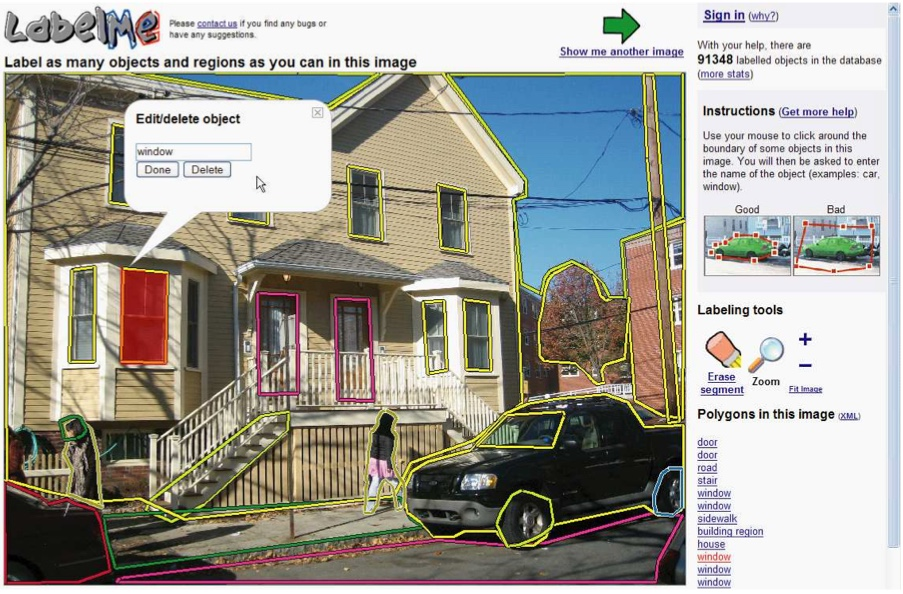
\includegraphics[width=\textwidth]{images/dataset/tools/label_me}
  \caption[The LabelMe user interface]{The LabelMe user interface \citep{Russell:2008wm}.}
  \label{}
\end{figure}

\paragraph{\glsac{apep}} 

\citet{Karatzas:2014bt} introduced the \glsac{cvc} \gls{apep}\footnoteurl{http://labelme.csail.mit.edu/}{17 August 2017}, made popular for use using the \gls{icdar} 2011--2015 Robust Reading Competitions. Unlike our system, users can edit the per-pixel boundaries using a `flood-fill' or `magic-select' markup tool (with an adjustable tolerance), followed by a skeletonisation of the boundaries filled. This speeds up selection of specific text areas quite useful (see Figure~\ref{}). While we did not incorporate a feature into Argus, a potential future version would benefit using such an annotation tool for a polygon, rather than clicking $n_{vertices}$ times if the vertices count is unknown. This could also be encoded using \gls{rle} as suggested from the \gls{coco} format in Section~\ref{sec:dataset:metamodel_evaluation:annotations}. Additionally, users are able to zoom into the photo to get finer accuracies at the pixel level.


\begin{figure}[h]
  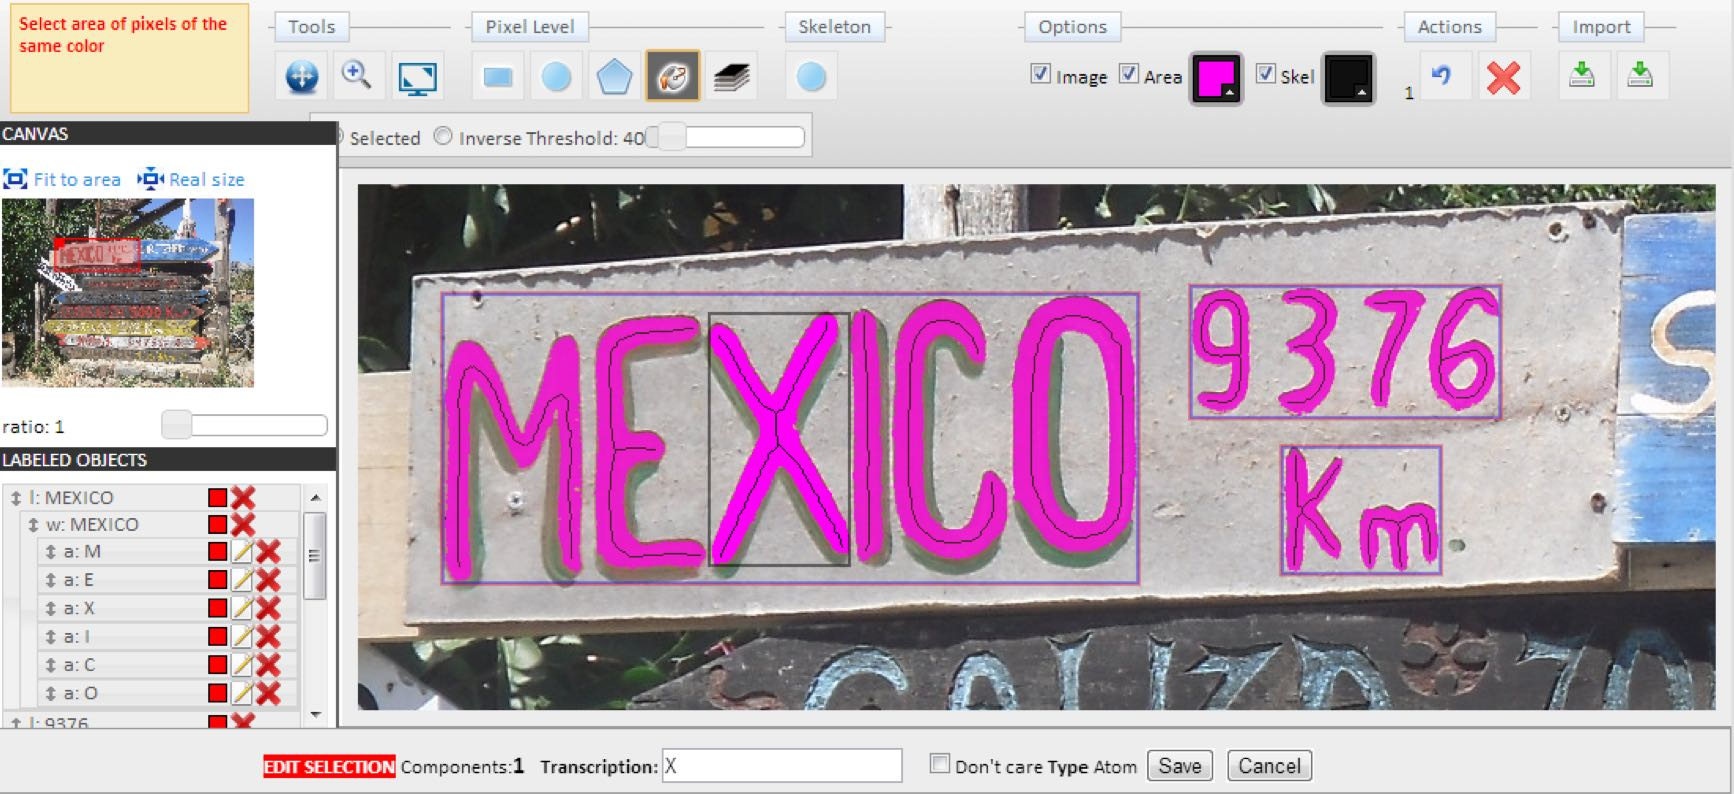
\includegraphics[width=\textwidth]{images/dataset/tools/apep}
  \caption[The APEP user interface]{The APEP ground truthing tool, showing a hierachy of textual content and defined text parts (flood-filled areas and skeletons) \cite{Karatzas:2014bt}.}
  \label{}
\end{figure}

% Robust Reading Competition by the Computer Vision Centre: http://www.cvc.uab.es/apep/images/DAS2014_Toolbox.pdf
% ICDAR12-15 which uses CVC Annotation and Performance Evaluation Platform (APEP) \cite{Karatzas:2015tj}

\paragraph{\glsac{amt}}

\gls{amt}\footnoteurl{https://www.mturk.com/mturk/welcome}{11 August 2017} provides \gls{saas} that does not require downloading or setting up (typically laborious for annotators). Annotation is achieved in the form of customised \glspl{hit}, using a custom interface. Recently, this is typically the most popular choice of annotation outsourcing \citep{Lin:2014vma,Veit:2016vj,Chen:2015ur,JiaDeng:2009dl,Netzer:2011to} due to flexibility in developing customised interfaces for the task at hand, though the benefits of ensuring a user-friendly crowdsourcing annotation system are presented by \citet{Matera:2014wq}. \citet{Sorokin:2008uk} discuss the utility of using \gls{amt} for annotation.

\paragraph{\glsdisp{vatic}{VATIC}}

\glsdisp{vatic}{VATIC (the \glsdesc{vatic})} is a a free web-based product developed by \citet{springerlink:10.1007/s11263-012-0564-1}, running on \gls{amt}. We note this tool specifically for the use of annotating video stills within an image: its intended purpose is for the sole use of object tracking in videos. There are only three annotations per object: the object name, the object is out of view, and the object is obstructed. It is useful in that not all frames have to be individually annotated, as the tool uses object tracking to estimate the movement between every 2-3 seconds. This may be useful to incorporate into future works of Argus. 

\begin{figure}[p]
  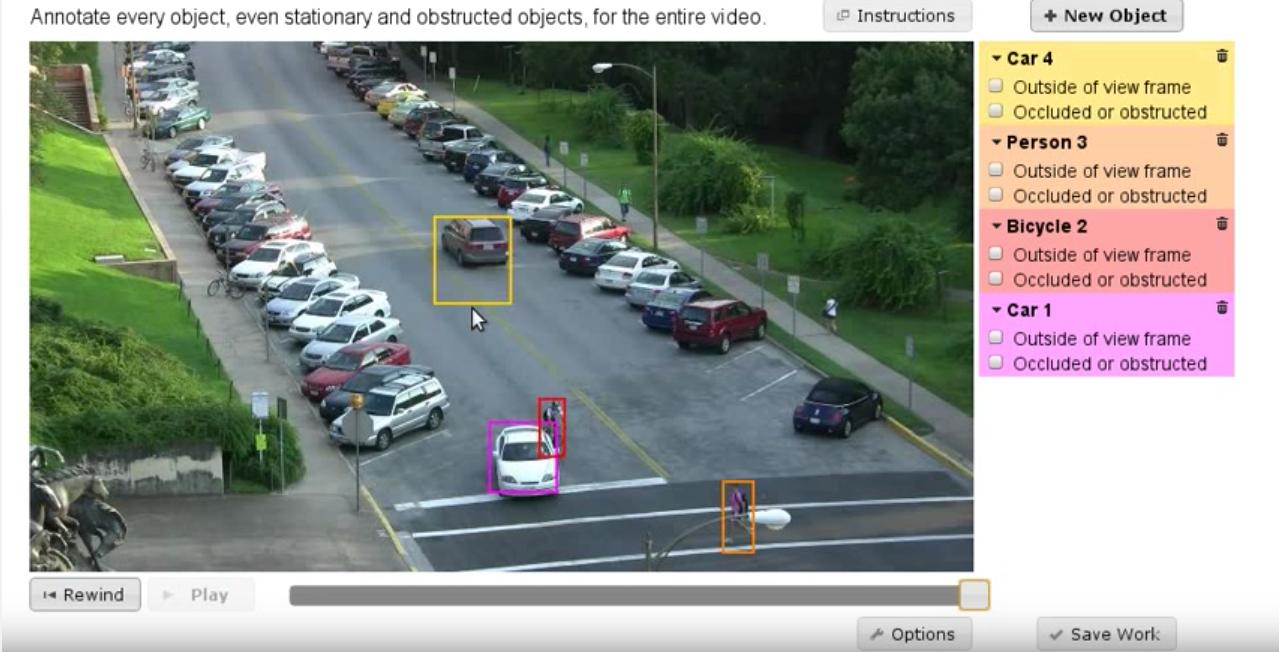
\includegraphics[width=\textwidth]{images/dataset/tools/vatic}
  \caption[The VATIC web-based user interface]{The \gls{vatic} web-based user interface. Sourced from \url{https://github.com/cvondrick/vatic}. (Last viewed 11 August, 2017.)}
\end{figure}

% - http://carlvondrick.com/vatic/ -> amazon turk
%% Only for object tracking in videos
%% No annotations, only two attributes per feature: (outside view frame or obfuscated)
%% Cannot label each feature, it's Car 1, Car 2, Car 3... may be hard for long videos. 
%% Useful in that you do not need to process every frame
%% PAPER: Utility data annotation with amazon mechanical turk

\paragraph{ScaleAPI}

ScaleAPI\footnoteurl{http://www.scaleapi.com}{11 August 2017} is a recent \gls{saas} that provides a web-based \gls{api} to return human-marked annotation in realtime. Various boundary annotations can be made on an image. Listings~\ref{lst:dataset:evaluation:scaleapi:req} and \ref{lst:dataset:evaluation:scaleapi:res} show the request and response for a simple instruction to draw bounding boxes around all pedestrians and cars in the image\footnoteurl{https://docs.scaleapi.com/?shell\#bounding-box-annotation}{17 August 2017}. Additionally, object segmentation (on a per-pixel basis). While there is no need for workflows in a single request (as multiple requests can be made for multiple workflow steps), instructions to annotators are provided on a per-request basis. Furthermore, ScaleAPI allows for categorisation and comparison tasks, data collection, \gls{ocr} and audio transcription.

\begin{lstlisting}[language=CURL, label=lst:dataset:evaluation:scaleapi:req, caption={[Sample ScaleAPI request] A sample ScaleAPI HTTP request made using cURL\footnotemark.}]
curl "https://api.scaleapi.com/v1/task/annotation" \
  -u "SCALE_API_KEY:" \
  -d callback_url="http://www.example.com/callback" \
  -d instruction="Draw a box around each **car** and **pedestrian**." \
  -d attachment_type=image \
  -d attachment="http://i.imgur.com/XOJbalC.jpg" \
  -d objects_to_annotate="car" \
  -d objects_to_annotate="pedestrian" \
  -d with_labels=true \
  -d min_width="30" \
  -d min_height="30"  
\end{lstlisting}
\footnotetext{\url{https://curl.haxx.se/} last accessed 17 August 2017.}

\begin{lstlisting}[language=JSON, label=lst:dataset:evaluation:scaleapi:res, caption={[Sample ScaleAPI response] Sample \glsac{json} response from the request made in Listing~\ref{lst:dataset:evaluation:scaleapi:req}.}]
{
  "task_id": "5774cc78b01249ab09f089dd",
  "created_at": "2016-9-03T07:38:32.368Z",
  "callback_url": "http://www.example.com/callback",
  "type": "annotation",
  "status": "pending",
  "instruction": "Draw a box around each **car** and **pedestrian**",
  "urgency": "day",
  "params": {
    "with_labels": true,
    "min_width": 30,
    "min_height": 30,
    "objects_to_annotate": [
      "car",
      "pedestrian"
    ],
    "attachment_type": "image",
    "attachment": "http://i.imgur.com/XOJbalC.jpg"
  },
  "metadata": {}
}
\end{lstlisting}
\clearpage

% - https://docs.scaleapi.com/#polygon-annotation
%% Large annotation 
%% Annotation as a service
